\documentclass[a4paper,10pt]{ctexart} %ctexart
%\usepackage{ctex}
%\usepackage{color}
%\usepackage{lineno} %打印行号的宏包,使用{linenumbers*}环境。
\usepackage[backref,hidelinks]{hyperref} %hidelinks去掉引用处的红框
\pagestyle{plain} %把页码从右上角移到页脚
%==========打印代码的设置===================
\usepackage{color}
\definecolor{gray}{rgb}{0.8,0.8,0.8}
\usepackage{listings}
\lstset{basicstyle=\small}
\lstset{numbers=left} \lstset{language=C++} \lstset{breaklines}
\lstset{extendedchars=false} \lstset{backgroundcolor=\color{gray}}
\lstset{keywordstyle=\color{blue}\bfseries} \lstset{frame=none}
\lstset{tabsize=4} \lstset{commentstyle=\color{red}}
\lstset{stringstyle=\emph}
%=======================================
\begin{document}
\begin{center}
{\Large\textbf{阶段汇报}}\\	%反过来嵌套就显示不出字.
\textbf{2016.4}
\end{center}

%\begin{flushright}
%\textbf{2016.4}
%\end{flushright}

\noindent \textbf{系统结构}\\
\begin{figure}[!htb]\center
%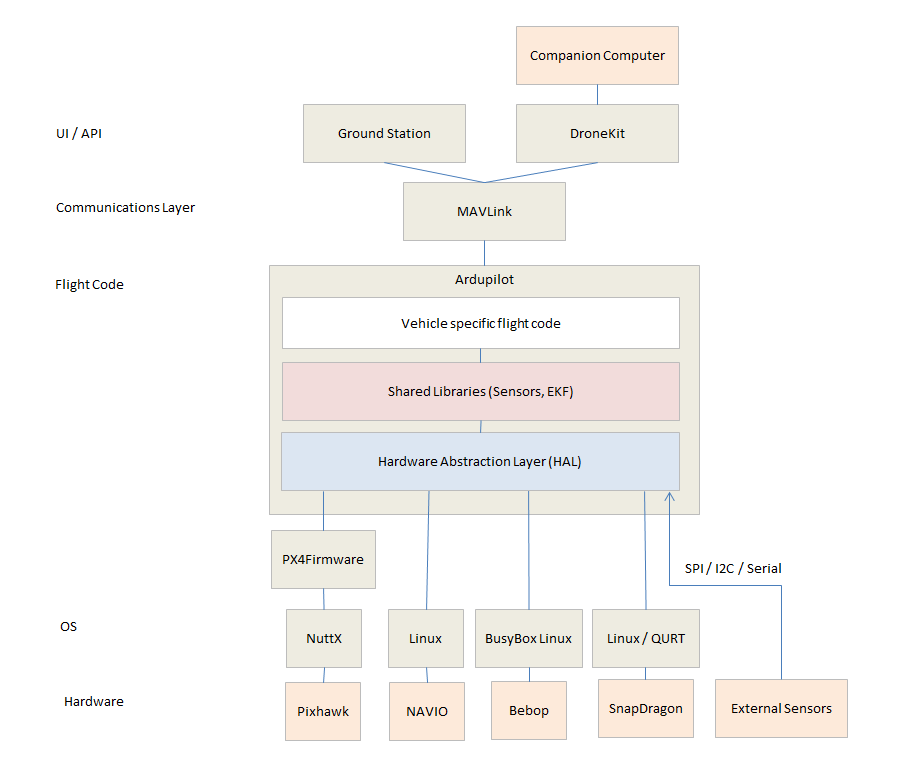
\includegraphics[scale=0.4]{pics/ArduPilot_HighLevelArchecture.png}
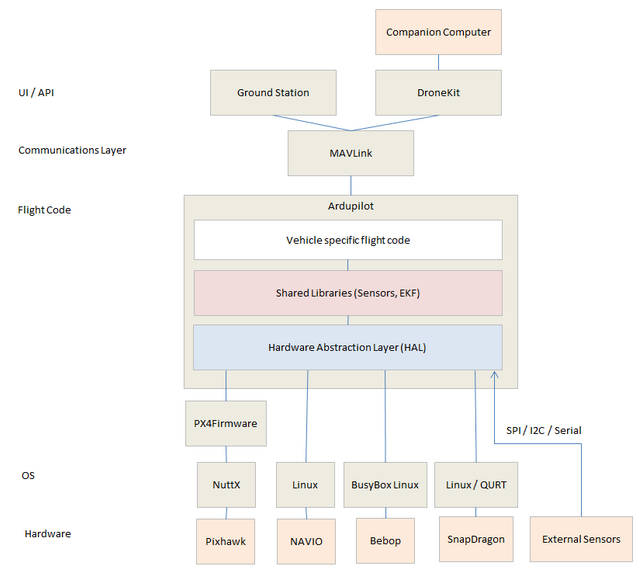
\includegraphics[scale=0.5]{pics/1.png}		%不清楚!
\caption{系统结构图}\label{figure1}
\end{figure}

主要组成:
\begin{itemize}
\item ArduCopter
\item libraries
\item HAL(AP\_HAL \& AP\_HAL\_PX4)
\item 外部模块(PX4Firmware,NuttX,uavcan,mavlink)
\end{itemize}

\vspace{20pt}
%=======================================
\noindent \textbf{串口定义}\\

包含USB接口在内,pixhawk共有6个串口。具体定义如下表:
\begin{table}[h] \centering   %h保证浮动体放置在当前位置上,\centering 使表格居中
\caption{串口定义}
\begin{tabular}{c|c|c|c|c}\hline
序号 & UART定义  &	  外部定义		   &  默认tty设备  &	波特率 \\\hline
 0	&	UARTA	&	 USB			&	/dev/ttyACM0	&	115200 \\
 1	&	UARTC	&	 telem1			&	/dev/ttyS1	&	57600 \\
 2	&	UARTD	&	 telem2			&	/dev/ttyS2	&	57600 \\
 3	&	UARTB	&	1st GPS			&	/dev/ttyS3	&	38400 \\
 4	&	UARTE	& serial4(2nd GPS)	&	/dev/ttyS6	&	38400 \\
 5	&	UARTF	&	serial5			&	/dev/null	&	57600 \\\hline
\end{tabular}\label{table1}
\end{table}

其中,serial5是底层操作系统nuttx默认的控制台(Console),
打印系统启动信息,并可作为NSH终端供手动控制操作系统中程序的运行。
serial5通过USB-TTL连接linux终端时对应的设备为\textbf{/dev/ttyUSB0}。

USB口是ArduPilot程序的默认控制台,在ArduPilot程序运行最初用于打印信息,
之后以Mavlink协议进行数据传输,通过USB线或数传与地面站通信。
\textit{某些情况下(如不插入SD卡启动),USB口也会被作为NSH终端使用。}

注意:\textbf{ArduPilot只是nuttx操作系统上运行的程序之一},
因此两个控制台的工作层面是不同的。
对两个串口的查看和操作,
在windows系统下,可使用任意串口程序或PX4 Toolchain自带程序TeraTerm;
在Linux系统下,可用的串口工具有screen、minicom等,
如可分别使用命令:
\textbf{screen /dev/ttyACM0 115200 8N1}
和\textbf{screen /dev/ttyUSB0 57600 8N1}
来打开USB口和serial5。

telem1\&2支持硬件流控制(RTS/CTS管脚)(主程序启动成功后被禁用)。

\vspace{20pt}
%=======================================
\noindent \textbf{主程序编译方式}\\

\noindent 主要命令:\\
\vspace{-20pt}
\begin{description}
\item[make px4-v2] 为pixhawk硬件编译固件;
\item[make px4-v2-upload] 编译固件并刷写;
\item[make px4-clean] 清理编译产生的部分文件;
\item[make px4-cleandef] 清理编译中使用的依赖文件(*.d);
\item[make sitl] 编译SITL软件。
\end{description}

\vspace{20pt}
%=======================================
\noindent \textbf{固件启动流程}\\

系统的引导由nsh脚本文件控制。
脚本文件最初位于ardupilot源程序的\textit{/mk/PX4/ROMFS/init.d}文件夹中,
编译时被存入固件,
最后刷写固件时存入pixhawk的Flash中(\textit{/etc/init.d})。
此文件夹中包含3个文件:\textbf{rcS},\textbf{rc.APM}和\textbf{rc.error}。

1.pixhawk启动时,自动运行rcS,LED灯启动并为白色:
\begin{lstlisting}
    # show startup white
    rgbled rgb 16 16 16
\end{lstlisting}
之后寻找microSD卡,找到则蜂鸣器发声:
\begin{lstlisting}
	tone_alarm /etc/tones/startup
\end{lstlisting}
否则,LED灯变为红色:
\begin{lstlisting}
    rgbled rgb 16 0 0
\end{lstlisting}
如果找到了MicroSD卡且对应位置有rc脚本文件,则运行脚本。

2.检查是否连接了USB。如果没有连接,则调用同目录下的rc.APM文件:
\begin{lstlisting}
    # if APM startup is successful then nsh will exit
    sh /etc/init.d/rc.APM
\end{lstlisting}
否则,将USB口设置为nsh终端:
\begin{lstlisting}
    nshterm /dev/ttyACM0 &
\end{lstlisting}

3.rc.APM的执行:首先进行硬件模块和各传感器的启动。
完成后,开始运行ArduPilot主程序:
\begin{lstlisting}
echo Starting ArduPilot $deviceA $deviceC $deviceD
if ArduPilot -d $deviceA -d2 $deviceC -d3 $deviceD start
then
    echo ArduPilot started OK
else
    sh /etc/init.d/rc.error
fi
\end{lstlisting}

4.如果脚本运行过程中出错,则调用rc.error,
LED灯变为红色,USB口被设置为NSH终端。
\begin{lstlisting}
	nshterm /dev/ttyACM0 &
\end{lstlisting}

\vspace{20pt}
%=======================================
\noindent \textbf{ArduPilot启动流程}\\

1.程序入口在主程序文件最后的宏定义。\\
\noindent 对于ArduCopter:
\begin{lstlisting}
	AP_HAL_MAIN_CALLBACKS(&copter);
\end{lstlisting}
对于其他测试例程:
\begin{lstlisting}
	AP_HAL_MAIN();
\end{lstlisting}
宏定义位于文件\textit{/libraries/AP\_HAL/AP\_HAL\_Main.h}中:
\begin{lstlisting}
#define AP_HAL_MAIN() extern "C" { \
	int AP_MAIN(void); \
	int AP_MAIN(void) { \
		AP_HAL::HAL::FunCallbacks callbacks(setup, loop);\
		hal.run(0, NULL, &callbacks); \
		return 0; \
	} \
}

#define AP_HAL_MAIN_CALLBACKS(CALLBACKS) extern "C" { \
	int AP_MAIN(void); \
	int AP_MAIN(void) { \
		hal.run(0, NULL, CALLBACKS); \
		return 0; \
	} \
}
\end{lstlisting}
即程序的真实起点为
\begin{lstlisting}
hal.run(0, NULL, &callbacks); 
\end{lstlisting}

2.要运行run()函数,首先程序需要获得hal:
\begin{lstlisting}
const AP_HAL::HAL& hal = AP_HAL::get_HAL();
\end{lstlisting}
(例子程序的此语句位于主程序文件开头,ArduCopter的此语句位于Copter.cpp而非主程序文件)。
对于pixhawk,hal对应的类型为AP\_HAL\_PX4。
函数get\_HAL()在AP\_HAL的每个子类中都有定义,
在编译时,系统使用了条件编译:
\begin{lstlisting}
#if CONFIG_HAL_BOARD == HAL_BOARD_PX4
\end{lstlisting}
从而只编译了PX4的一个子类AP\_HAL\_PX4,AP\_HAL::get\_HAL()的实现为:
\begin{lstlisting}
const AP_HAL::HAL& AP_HAL::get_HAL() {
    static const HAL_PX4 hal_px4;
    return hal_px4;
}
\end{lstlisting}
而全局搜索宏CONFIG\_HAL\_BOARD,并没有找到其定义。
实际上,这个宏定义是通过makefile中的-D选项实现的:

\begin{lstlisting}
	SKETCHFLAGS=$(SKETCHLIBINCLUDES) ……
	 	-DCONFIG_HAL_BOARD=HAL_BOARD_PX4 ……
\end{lstlisting}
此语句存在于mk/PX4\_target.mk,其调用逻辑为:\\
(1)编译时所在目录的makefile调用/mk/apm.mk;\\
(2)/mk/apm.mk调用/mk/environ.mk;\\
(3)/mk/environ.mk利用变量MAKECMDGOALS(即输入make命令时的参数,如px4-v2),
将变量HAL\_BOARD定义为HAL\_BOARD\_PX4;\\
(4)/mk/apm.mk根据变量HAL\_BOARD调用/mk/board\_px4.mk;\\
(5)/mk/board\_px4.mk调用/mk/px4\_target.mk。

AP\_HAL\_PX4类的run()函数位于文件HAL\_PX4\_Class.cpp:
\begin{lstlisting}
void HAL_PX4::run(int argc, char * const argv[], Callbacks* callbacks) const
\end{lstlisting}
函数的输入参数(argv[ ])为脚本文件rc.APM调用ArduPilot时的参数:
\begin{lstlisting}
ArduPilot -d $deviceA -d2 $deviceC -d3 $deviceD start
\end{lstlisting}

3.run()函数通过创建nuttx操作系统任务的方式(px4\_task\_spawn\_cmd()),
建立一个守护进程(daemon\_task),
用于运行main\_loop()函数:
\begin{lstlisting}
daemon_task = px4_task_spawn_cmd(SKETCHNAME,
                                SCHED_FIFO,
                                APM_MAIN_PRIORITY,
                                APM_MAIN_THREAD_STACK_SIZE,
                                main_loop,
                                NULL);
\end{lstlisting}
在nsh中可通过ps命令显示操作系统上运行的进程,
此守护进程的名字为所编译程序的名字(SKETCHNAME,如ArduCopter(),UART\_test()),
优先级(PRI)为180。

4.main\_loop()函数首先为ArduPilot进行一系列初始化设置:
\begin{lstlisting}
    hal.uartA->begin(115200);
    hal.uartB->begin(38400);
    hal.uartC->begin(57600);
    hal.uartD->begin(57600);
    hal.uartE->begin(57600);
    hal.scheduler->init();
    hal.rcin->init();
    hal.rcout->init();
    hal.analogin->init();
    hal.gpio->init();	
\end{lstlisting}
其中需特别注意scheduler的初始化。在HAL\_PX4\_Class.cpp中发现,
init()函数创建了4个新的线程:
\begin{lstlisting}
// setup the timer thread - this will call tasks at 1kHz
pthread_create(&_timer_thread_ctx, &thread_attr, &PX4Scheduler::_timer_thread, this);
// the UART thread runs at a medium priority
pthread_create(&_uart_thread_ctx, &thread_attr, &PX4Scheduler::_uart_thread, this);
// the IO thread runs at lower priority
pthread_create(&_io_thread_ctx, &thread_attr, &PX4Scheduler::_io_thread, this);
// the storage thread runs at just above IO priority
pthread_create(&_storage_thread_ctx, &thread_attr, &PX4Scheduler::_storage_thread, this);
\end{lstlisting}
这些线程分别进行计时器、UART、IO和存储的操作。
在NSH终端利用ps命令,打印出各线程的具体信息,如下表:
\begin{table}[h] \centering   %h保证浮动体放置在当前位置上,\centering 使表格居中
\caption{操作系统进程列表}
\begin{tabular}{c|c|c|c|c|c|c}\hline
PID & PRI & SCHD & TYPE    & NP & STATE & NAME \\\hline
 0  &  0  & FIFO & TASK    &    & READY & Idle Task() \\
 1  & 192 & FIFO & KTHREAD &    & WAITSEM & hpwork() \\
 2  &  50 & FIFO & KTHREAD &    & WAITSIG & lpwork() \\
 3  & 100 & FIFO & TASK    &    & RUNNING & init() \\
10  & 240 & FIFO & TASK    &    & WAITSEM & px4io() \\
43  & 180 & FIFO & TASK    &    & WAITSEM & ArduCopter() \\
44  & 181 & FIFO & PTHREAD &    & WAITSEM & <pthread>(20003b70) \\
45  & 60  & FIFO & PTHREAD &    & WAITSEM & <pthread>(20003b70) \\
46  & 58  & FIFO & PTHREAD &    & WAITSEM & <pthread>(20003b70) \\
47  & 59  & FIFO & PTHREAD &    & WAITSEM & <pthread>(20003b70) \\\hline
\end{tabular}\label{table2}
\end{table}

\noindent 最后4个线程即hal.scheduler->int()创建的线程,
其PID是连续的,因为它们由守护进程(PID=43)依次创建。
其名字为<pthread>(XXX),XXX是hal.scheduler的首地址。
多线程的运用,可以更好地调度执行速度慢的任务(如读写MicroSD卡)而不影响核心飞控程序的运行。

%(运行例子程序时,需注释掉rcin,rcout,analogin,gpio初始化中的部分或全部语句,否则程序无法运行。)\\
\noindent 之后,降低守护进程的优先级并调用主程序的setup()函数:
\begin{lstlisting}
/*
  run setup() at low priority to ensure CLI doesn't hang the
  system, and to allow initial sensor read loops to run
 */
hal_px4_set_priority(APM_STARTUP_PRIORITY);

schedulerInstance.hal_initialized();

g_callbacks->setup();
hal.scheduler->system_initialized();

perf_counter_t perf_loop = perf_alloc(PC_ELAPSED, "APM_loop");
perf_counter_t perf_overrun = perf_alloc(PC_COUNT, "APM_overrun");
struct hrt_call loop_overtime_call;

thread_running = true;
\end{lstlisting}
最后,恢复守护进程的优先级,循环调用loop()函数:
\begin{lstlisting}
/*
  switch to high priority for main loop
 */
hal_px4_set_priority(APM_MAIN_PRIORITY);

while (!_px4_thread_should_exit) {
	……
    g_callbacks->loop();
	……
	
    /*
      give up 250 microseconds of time, to ensure drivers get a
      chance to run. This relies on the accurate semaphore wait
      using hrt in semaphore.cpp
     */
    hal.scheduler->delay_microseconds(250);
}
\end{lstlisting}

\vspace{20pt}
%=======================================
\noindent \textbf{常用的hal函数}\\
\begin{itemize}
\item hal.console(或uartA...E)->printf(),print(),println()
\item hal.scheduler->millis(),micros():系统启动以来的时间
\item hal.scheduler->delay(),delay\_microseconds():休眠
\item hal.gpio->pinMode(),read(),write()
\item hal.i2c
\item hal.spi
\end{itemize}
详细的接口函数参考硬件抽象层函数库AP\_HAL\_PX4。

\vspace{20pt}
%=======================================
\noindent \textbf{PX4系统控制台}\\

前面已经提到,可通过两种方式操作系统控制台:
直接使用串口5;或拔出SD卡,连接USB。
进入控制台,界面显示nsh>,此时可进行命令行操作。
输入help可显示所有命令和刷入的程序(Builtin Apps)。
常用命令包括:
ls列出文件结构(不支持输入参数);
ps列出正在运行的进程。
内嵌程序包括各硬件模块的驱动程序和主程序ArduPilot,
可对各传感器进行启动(start)、停止(stop)和测试(test)等操作。







%=======================================





\begin{flushright}
\vspace{30pt}
2016.4.25\\
方酉
\end{flushright}
\end{document}